\section{Langages de programmation}
Cette partie traite des différents éditeurs et langages de programmation utilisés dans les organisations présentées au point précédent.
\subsection{Blockly}
\label{blockly}
\begin{figure}[!h]
  \begin{center}
    
\includegraphics[scale=0.5]{content/5-related_work/images/blocky}
    \caption{Logo de Blocky}
    \label{fig:blocky}
  \end{center}
\end{figure}
Blockly\footnote{\url{https://code.google.com/p/blockly/}} est un langage de programmation graphique basé sur des technologies du web. 

Blockly est influencé\footnote{\url{https://code.google.com/p/blockly/wiki/Alternatives}} par "App Inventor" qui est influencé par "Scratch", lui-même influencé par "StarLogo"\footnote{\url{http://education.mit.edu/starlogo/}}.\\

Blockly a comme particularité :
\begin{itemize}
\item de s'exécuter dans un navigateur ;
\item d'exporter du code source en JavaScript, Dart, etc. ;
\item d'être open source ;
\item d'être haut niveau.
\end{itemize}

Il n'est pas directement une plateforme d'éducation dans le sens où, il peut être utilisé autant pour l'éducation, le business, des jeux, \ldots en fonction des blocs implémentés.\\

Blockly a été conçu avec certaines propriétés choisie lors de sa création. Les trois premières augmentent la compréhension des néophytes, les autres portent sur des facilités du langage. Les propriétés décidées lors de la conception du langage sont\footnote{\url{https://code.google.com/p/blockly/wiki/Language}} :

\begin{itemize}
  \item des indices de listes commençant à 1 ;
  \item des noms de variables non sensibles à la casse ;
  \item pas de portée de variable, elles sont toutes globales ;
  \item la possibilité de faire un export en JavaScript ;
  \item un code natif généré proche de celui des blocs.
\end{itemize}

\subsection{Scratch 1}
\begin{figure}[!h]
  \begin{center}
    
\includegraphics[scale=0.4]{content/5-related_work/images/scratch}
    \caption{Logo de Scratch}
    \label{fig:scratch}
  \end{center}
\end{figure}
Scratch est un langage de programmation graphique développé par le MIT pour apprendre aux enfants la programmation. C'est l'interface qui permet de faire des scripts facilement grâce à une programmation par blocs et du glisser-déposer.\\

Il a été pensé pour être un outil créatif pour réaliser des histoires, des jeux, des simulations, de l'art, etc. Il a, par exemple, son propre éditeur d'image et de sons. Un autre but de ce langage est d'être simple à utiliser et à apprendre. Il a en effet été conçu pour des enfants n'ayant aucune connaissance préalable en programmation.\\

Actuellement Scratch est à sa version 2 qui est une version web. Cette version a été complètement réécrite en flash par rapport à la version 1 en Smalltalk. De plus, la version 2 n'est plus open source contrairement à la première version.

Comme le montre la figure \ref{fig:scratch-printscreen}, l'interface de Scratch se divise en plusieurs grandes parties :
%TODO image scratch
\begin{enumerate}
\item sur la gauche, il y a la zone de dessin dans laquelle s'anime les composants graphiques des scriptes ;
\item au milieu, une liste des blocs disponible triés par catégorie ;
\item sur la droite, la zone de scripte qui contient tous les scriptes liés au sprite sélectionné.
\end{enumerate}
\begin{figure}[!h]
  \begin{center}
    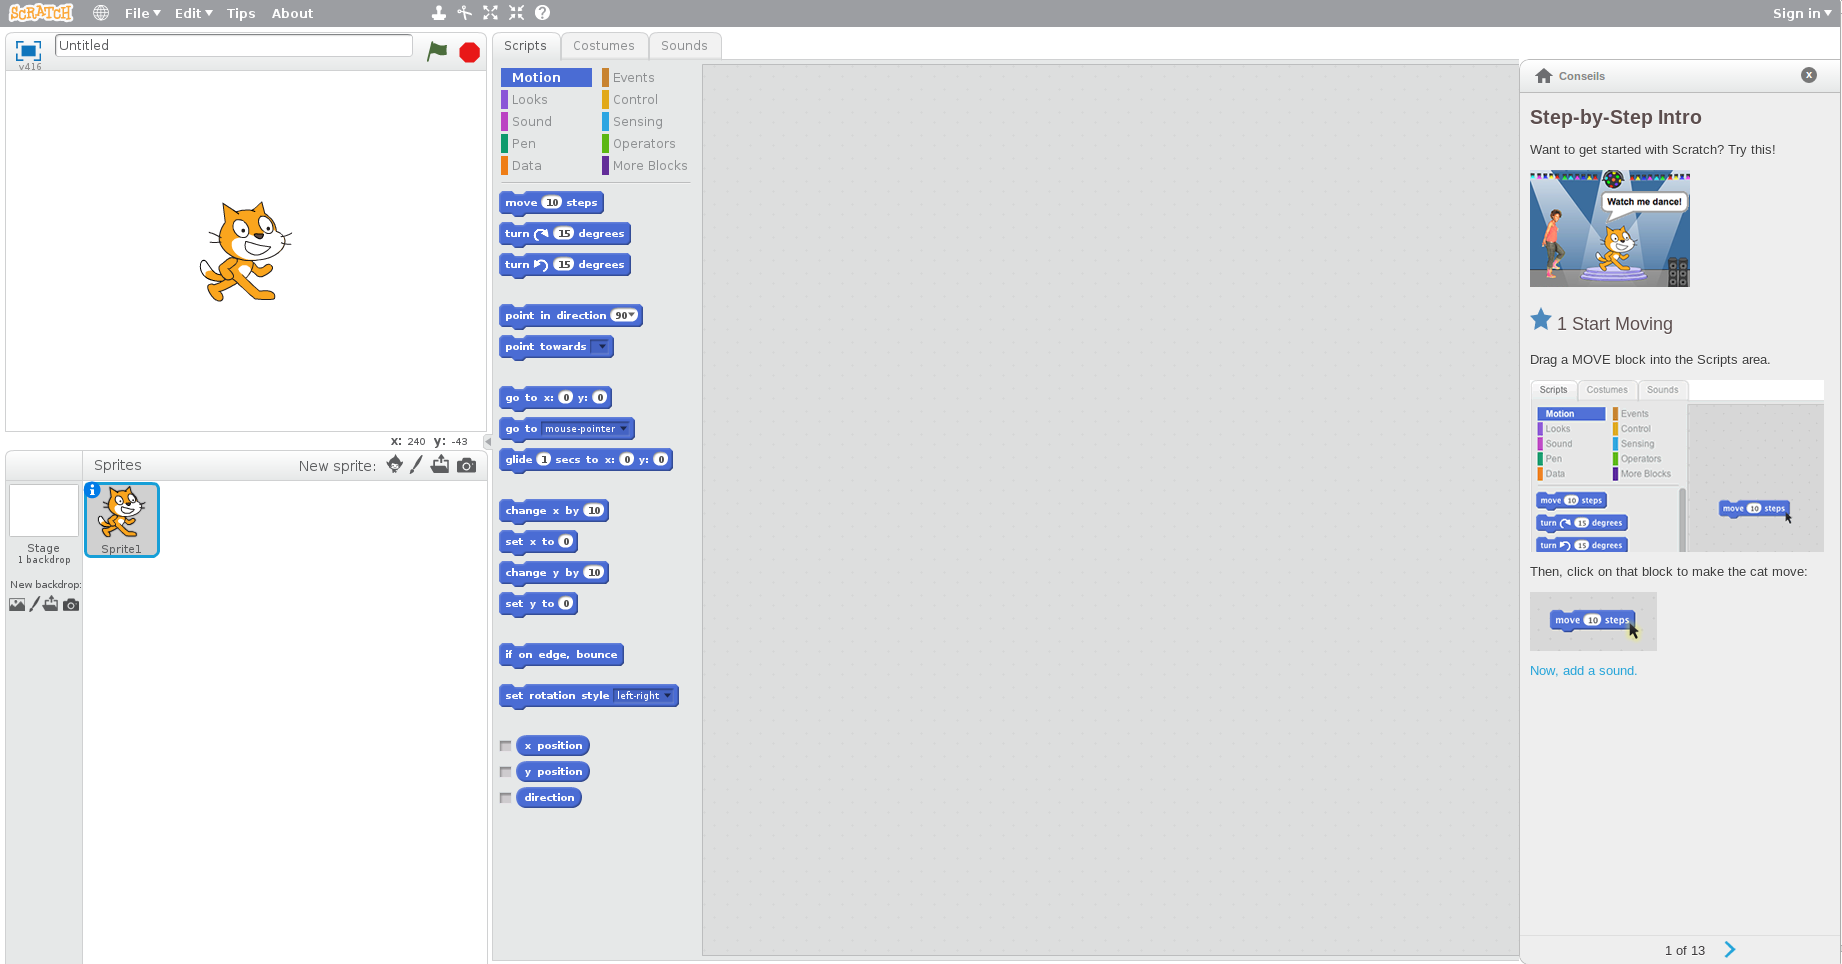
\includegraphics[scale=0.2]{content/5-related_work/images/scratch-printscreen}
    \caption{Interface de Scratch}
    \label{fig:scratch-printscreen}
  \end{center}
\end{figure}

\subsection{SNAP!}
\begin{figure}[!h]
  \begin{center}
    
\includegraphics[scale=0.07]{content/5-related_work/images/snap}
    \caption{Logo de SNAP!}
    \label{fig:snap}
  \end{center}
\end{figure}
SNAP est un langage de programmation de "glissé-déposé" de blocs. C'est une ré-implémentation et une extension du langage Scratch du MIT. Il a été pensé et conçu pour être orienté web. Il est donc implémenté en JavaScript.\\

Ce langage est né en 2011 et a été créé par Jens Mönig. Il se distingue de son père Scratch par l'ajout :
\begin{enumerate}
\item de fonctions et de procédures de première classe ;
\item de listes de première classe ;
\item de sprite de première classe.
\end{enumerate}

\subsection{Python}
\begin{figure}[!h]
  \begin{center}
    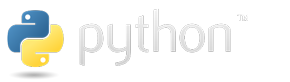
\includegraphics[scale=0.4]{content/5-related_work/images/python}
    \caption{Logo de Python}
    \label{fig:python}
  \end{center}
\end{figure}
Python est un langage de programmation qu'il ne faut plus présenter. Il a beaucoup d'avantages dont celui d'avoir une syntaxe légère et d'être facile à prendre en main. Une grande communauté et beaucoup de bibliothèques, dont la fameuse \texttt{turtle}, en fait un excellent langage pour démarrer dans la programmation.

Cependant, devoir apprendre un langage de programmation et la logique informatique en même temps complique la tâche. De plus, lorsqu'on commence un nouveau langage de programmation il faut également apprendre ses bonnes pratiques de codage. %TODO réécrire de manière neutre

C'est donc un langage qui ne convient pas aux trop jeunes ni à ceux qui ne sont pas vraiment investis dans l'apprentissage de la programmation.
